\documentclass[a4paper, 11pt]{article}



\usepackage[utf8]{inputenc} 
\usepackage[T1]{fontenc}
\usepackage{lmodern}
\usepackage{graphicx}
\usepackage[french]{babel}
\usepackage{color}
\usepackage{fullpage}
\usepackage{array}
\usepackage[tight]{shorttoc}
\usepackage[toc,page]{appendix} 
\usepackage{makeidx} 

\definecolor{gris}{gray}{0.45}

\newcommand{\rouge}[1]{\textcolor{red}{#1}}
\newcommand{\rem}[1]{\textcolor{blue}{\emph{Remarque: \\} #1}}
\newcommand{\exl}[1]{\textcolor{gris}{\emph{Exemple: } #1}}
\newcommand{\exc}[1]{\textcolor{gris}{(\emph{Ex:} #1)}}
\newcommand{\cod}[1]{\textcolor{gris}{\emph{#1}}} 
\newcommand{\att}[1]{\textcolor{red}{\emph{\\ Attention: \\} #1 \\}}

\usepackage{listings}
\definecolor{dkgreen}{rgb}{0,0.6,0}
\definecolor{gray}{rgb}{0.5,0.5,0.5}
\definecolor{mauve}{rgb}{0.58,0,0.82}
\definecolor{red}{rgb}{1,0,0}

\newcommand{\lstconfig}[1]{
	\lstset{
	  language=#1,				      % the language of the code
	  basicstyle=\footnotesize,	      % the size of the fonts that are used for the code
	  numbers=left,				      % where to put the line-numbers
	  numberstyle=\footnotesize,	  % the size of the fonts that are used for the line-numbers
	  stepnumber=1,				      % the step between two line-numbers. If it's 1, each line 
									  % will be numbered
	  numbersep=5pt,				  % how far the line-numbers are from the code
	  backgroundcolor=\color{white},  % choose the background color. You must add \usepackage{color}
	  showspaces=false,			      % show spaces adding particular underscores
	  showstringspaces=false,		  % underline spaces within strings
	  showtabs=false,				  % show tabs within strings adding particular underscores
	  frame=single,				      % adds a frame around the code
	  tabsize=2,					  % sets default tabsize to 2 spaces
	  captionpos=b,				      % sets the caption-position to bottom
	  breaklines=true,				  % sets automatic line breaking
	  breakatwhitespace=false,		  % sets if automatic breaks should only happen at whitespace
	  title=\lstname,	   			  % show the filename of files included with \lstinputlisting;
									  % also try caption instead of title
	  numberstyle=\tiny\color{gray},  % line number style
	  keywordstyle=\color{blue},	  % keyword style
	  commentstyle=\color{dkgreen}\textit,   % comment style
	  stringstyle=\color{mauve}\textbf,	  % string literal style
	}
}

	\title{\vspace{5cm}SmallWorldUtbm \\ Rapport de projet \\ \ \\}
	\date{automne 2012\\ \ \\ \vspace*{3cm}
	\includegraphics[width=4cm]{logo_utbm.png}
	}
	\author{Amani Younes - Michael Longo - Gabriel Notong - Pierre Rognon \\ \ \\ \ \\ Université de Technologies de Belfort-Montbéliard\\ \ \\}
	
\renewcommand{\appendixtocname}{Annexes}
\renewcommand{\appendixpage}{\huge \textbf{Annexes} \normalsize}
\renewcommand{\appendixname}{{\sffamily Annexe}} 	

\begin{document}

	
	\maketitle
	
	\newpage
	
	\shorttoc{Sommaire}{1}
	
	\newpage
	
	\section*{Introduction}
	
	Dans le cadre de l'Unité de Valeur LO43, il a été demandé aux étudiants de réaliser un projet de fin de semestre. Ce projet a pour but de mettre en application les différentes notions acquises en programmation orientée objet ainsi que de pratiquer un langage de programmation: le Java. L'objectif de ce projet est de créer un jeu de rôle à partir d'un jeu de société existant.
	\paragraph{} SmallWorld est un jeu de stratégie se rapportant à l'univers fantastique. A partir d'un peuple légendaire choisi, il s'agit d'effectuer des conquêtes sur un plateau de jeu comportant des territoires. L'occupation de ces territoires permet alors de remporter de l'argent à chaque tour pour ensuite gagner la partie. 
	\paragraph{}A l'occasion de ce projet, le jeu a été renommé SmallWorldUtbm et il a été demandé d'appliquer les grands principes du jeu d'origine tout en l'adaptant à la vie Utbohémienne. \\
	Cette adaptation a donc demandé une organisation en plusieurs étapes qui seront présentées dans une première partie. Sera ensuite abordée la mise en œuvre de ce projet comprenant des détails sur la conception et le développement de l'application. Enfin, les problèmes rencontrés et un bilan succin seront dressés.
	
	
	\newpage
	
	\section{Cahier des charges}
	
	Le cahier des charges impliquait plusieurs parties. En effet, le sujet portant sur un jeu existant, une première étape consiste à découvrir les règles du jeu et les entités liées à celui-ci puis à les adapter au projet. Suite à cela, une seconde étape porte sur la réalisation d'une modélisation dans le langage UML. Le cahier des charges concernant l'application concerne la troisième partie du travail.
	
		\subsection{Étude de l'existant et adaptation}
		
		L'étude de l'existant doit permettre de réaliser plusieurs choses. Tout d'abord, elle doit permettre de comprendre les différentes règles du jeu. Elle doit ensuite aider à dissocier les différentes entités relatives à celui-ci. Cela doit avancer une première fois la réflexion sur la réalisation de l'application. \\
		L'adaptation au sujet proposé est en lien direct avec l'existant. Elle doit en effet reprendre les grandes idées de l'existant tout en calquant les entités de l'UTBM. Cette adaptation doit être en réalité une sorte de première étape de conception puisqu'elle met déjà en jeu les différentes entités qui seront rassemblées lors de la conception proprement dite.
			
		\subsection{Conception}
		
		Pour la conception, le cahier des charges est en grande partie donné et la marge de manœuvre est faible. On doit donc réaliser:
		\begin{itemize}
			\item des diagrammes de cas d'utilisation;
			\item des diagrammes de séquence;
			\item un diagramme de classes.
		\end{itemize}
		Cette étape de conception s'appuie grandement sur l'adaptation faite lors de l'étude de l'existant. Les entités doivent en effet déjà avoir été isolées pour réaliser l'adaptation à notre contexte. L'étape de conception doit donc simplement transférer ces idées en respectant la syntaxe et les normes UML. Le diagramme de classes doit aussi permettre de développer plus facilement par la suite les classes Java en étant donc assez précis. \\ \ \\
		Suite à cela est réalisé le cahier des charges dit fonctionnel de l'application. Il permettra le développement de celle-ci.
		
		\subsection{Application}
		
		Le cahier des charges de l'application indique ce que devra faire celle-ci en développant son comportement. Un certain nombre de choses à faire sont donc déjà énoncées par le sujet ou par l'existant mais d'autres sont à indiquer. Ces besoins sont énumérés ci-dessous en quatre parties: tout d'abord ceux relatifs à un début de partie, ensuite d'autres en liens avec le cours de la partie, puis les besoins intervenant en fin de partie. Une dernière partie traitera des besoins liés à l'interface.
		
			\paragraph{Début de partie\\}
			
			L'application doit répondre à un certain nombre de besoins en début de partie. \\
			
			Tout d'abord, un certain nombre de règles générales ont été établies :
			\begin{itemize}
				\item l'application doit permettre d'effectuer des parties avec un nombre de joueur variables (de 2 à 4 joueurs);
				\item différents plateaux de jeu doivent être disponibles en fonction du nombre de joueurs dans une partie;
				\item on doit pouvoir choisir le nom des joueurs;
				\item l'application doit permettre au joueur de choisir un couple Peuple/Pouvoir; \\
			\end{itemize}
			
			Pour cette application, un grand nombre de traitements se font de façon transparente par rapport au joueur. Ceux-ci sont traduits par les besoins suivants:
			\begin{itemize}
				\item l'application doit initialiser tous les peuples disponibles ainsi que les pouvoirs;
				\item elle doit générer des couples aléatoires peuple/pouvoir afin que le joueur en choisisse une;
				\item les territoires doivent être générés ainsi que les éléments potentiellement présents sur chacun d'eux;
				\item l'application doit gérer l'argent liée à chaque couple peuple/pouvoir puisqu'un joueur peut payer pour prendre un couple.
			\end{itemize}
			
			\paragraph{Cours de partie\\}
			
			Du coté de l'utilisateur, on a les besoins suivants:\\
			\begin{itemize}
				\item Pour la phase de conquête de territoires:
				\begin{itemize}
					\item il doit pouvoir tant qu'il n'a encore rien pris durant le tour cliquer sur un bouton de passage en déclin du peuple. Le joueur finit alors son tour directement;
					\item si le joueur a passé son peuple en déclin au tour précédent, l'application doit lui proposer de choisir un nouveau peuple lorsqu'il joue à nouveau;
					\item il doit pouvoir cliquer sur les territoires qu'il peut prendre (géographiquement);
					\item l'application dans ces deux cas demander confirmation au joueur;
					\item l'application doit proposer lorsque le joueur n'a pas assez de pions pour attaquer un territoire de lancer un dé: si il accepte, on doit alors passer à la phase suivante.
					\item le joueur doit pouvoir cliquer sur un bouton de fin de tour pour passer à la phase suivante. \\
				\end{itemize}
				\item Pour la phase de redéploiement:
				\begin{itemize}
					\item le joueur doit pouvoir cliquer sur tous ses territoires;
					\item l'application doit alors proposer le nombre de pions à placer sur celui-ci;
					\item le joueur doit pouvoir cliquer sur un bouton de fin de redéploiement lorsqu'il a fini;
					\item l'application ne doit pas proposer de bouton de fin tant que le joueur a des pions dans les mains. \\
				\end{itemize}
				\item Pour la phase de redéploiement des autres joueurs, les besoins sont les même que pour celle du joueur qui vient d'effectuer son tour.	 \\	
			\end{itemize}

			En arrière-plan, l'application doit:
			\begin{itemize}
				\item ne permettre au joueur que de cliquer sur les territoires auxquels il peut accéder;
				\item calculer à chaque changement le nombre d'unités en main;
				\item effectuer les changements d'occupant pour les territoires abandonnés ou conquis;
				\item vérifier dans le cas où des joueurs ont des peuples en déclin que ceux-ci ont toujours des territoires. S'ils n'en n'ont plus, l'application doit supprimer le peuple en déclin du joueur et le remettre dans la liste des peuples libres;
				\item en fin de tour, calculer l'argent gagnés par le joueur. Ceux-ci sont calculés à partir des territoires occupés par son peuple mais aussi par ceux occupés par son peuple en déclin et en fonction de ses éventuels bonus.
			\end{itemize}
			
			\paragraph{Fin de partie\\}
			
			Pour l'utilisateur, l'application doit simplement indiquer quel est le gagnant de la partie. Le joueur doit pouvoir ensuite soit rejouer une partie, soit quitter le jeu. \\
			En arrière-plan, pour indiquer quel est le gagnant, l'application doit calculer quel joueur a le plus d'argent accumulés.
		
			\paragraph{Apparence et mise en page générale\\}
			
			La réalisation de cette application doit intégrer une interface graphique. Un certain nombre de règles sont donc à énoncer:\\
			
			\begin{itemize}
				\item l'interface doit fournir les informations suivantes au joueur lors de son tour dans un cadre d'informations sur le joueur dans un coin de la fenêtre de jeu. Les informations suivantes seront mises en évidence dans un liseret de la couleur décernée au joueur:
				\begin{itemize}
					\item le nom du joueur;
					\item son peuple actif ainsi que le pouvoir associé;
				\end{itemize}
				D'autres informations complétant les premières seront indiquées dans le cadre hors du liseret:
				\begin{itemize}
					\item l'argent possédée;
					\item le nombre d'unités totales qu'il possède;
					\item le nombre de territoires occupés à l'instant où il joue;
					\item le nombre d'unités qu'il a en main à l'instant où il joue;
					\item l'éventuel peuple en déclin qu'il possède. \\
				\end{itemize}
				
				\item elle doit aussi comprendre des informations sur les territoires mises à jour en fonction du territoire pointé par la souris. Ces informations, contenues dans un cadre d'information du territoire dans un coin de la fenêtre, sont:
				\begin{itemize}
					\item l'occupant du territoire;
					\item le nombre d'unités présentes sur celui-ci;
					\item le coût de l'attaque pour le joueur en train de jouer;
					\item les éventuels éléments que contient le territoire.
				\end{itemize}
				Le titre du cadre doit avoir pour fond la couleur décernée au joueur.
				\item les territoires doivent de plus indiquer sur leur espace le nombre d'unités contenues sur celui-ci. Ce chiffre doit être accompagné d'une couleur en arrière-plan correspondant à la couleur décernée au joueur. Si le peuple occupant est en déclin, la couleur sera adoucie; \\
				
				\item un dernier cadre dont le titre a aussi pour fond la couleur du joueur doit contenir les boutons suivants:
				\begin{itemize}
					\item fin du tour;
					\item passage en déclin du peuple;
					\item fin du redéploiement.
				\end{itemize}
				Ces boutons doivent être disponibles en fonction de l'étape de jeu du joueur. \\
				
				\item un cadre temporaire doit apparaître pour expliquer au joueur les différents choix impossibles lorsque celui-ci les tente. Ce cadre doit être bien visible et aura une couleur de police rouge. Il doit servir par exemple lorsque l'on clique sur un territoire impossible à attaquer à l'indiquer au joueur. \\
			\end{itemize}
			
			Des informations entre les étapes et les tours doivent aussi apparaître pour situer le joueur. Ces informations sont:
			\begin{itemize}
				\item une page temporaire indiquant l'étape de conquête du joueur en cours avant que celui-ci attaque des régions;
				\item une page temporaire affichant le redéploiement du joueur en cours;
				\item une page temporaire affichant le redéploiement des éventuels joueurs qui ont des unités en main suite à des pertes de territoires;
				\item enfin en fin de tour, une page temporaire indiquant l'argent durement acquis lors du tour du joueur.
			\end{itemize}
			
		\subsection{Contraintes et choix techniques}
		
		Le cahier des charges comprend différentes contraintes qui ont été imposées par le propos du sujet. D'autres contraintes ont été rajoutées par l'équipe. Ces différentes contraintes sont de différents types. \\
		
		De type temporel: 
		\begin{itemize}
			\item le rapport du projet doit être rendu pour le 4 janvier et le projet doit donc être terminé pour cette même date;
			\item les emplois du temps des différents membres du projet étant différents, des créneaux horaires en commun doivent être trouvés pour les réunions de projet. \\
		\end{itemize}
		
		De type technique:
		\begin{itemize}
			\item le langage de programmation est imposé: le Java;
			\item de plus, la bibliothèque graphique présentée en cours est Swing. C'est donc cette dernière qui doit être utilisée;
			\item afin d'éviter les problèmes de compatibilité, un environnement de développement est imposé: Eclipse. Il a l'avantage d'être largement utilisé et d'être disponible sur les systèmes d'exploitations les plus utilisés (Linux, Windows, MacOs);
			\item afin de pouvoir travailler chacun chez soi entre les différentes réunions, un gestionnaire de version est mis en place: Git. Ce dernier a été choisi car lié au site Github.com, il a l'avantage d'être simple à utiliser et de proposer des informations pratiques sur le développement. Le choix se justifie aussi du fait qu'un plugin liant Git à Eclipse est disponible. Ce dernier permet d'utiliser les deux en lien étroit et facilement;
			\item pour regrouper les éléments et les territoires du jeu, une base de données doit être utilisée: il a été choisi SQLite pour représenter cette base de données. SQLite présente l'intérêt de ne pas nécessiter de serveur et d'avoir une interface graphique pour créer la base de données. C'est aussi un système léger puisque ne générant qu'un fichier pour une base de données, il est portable et très répandu.
		\end{itemize}
		
		\newpage
		
	\section{Mise en œuvre}
	
		La mise en œuvre a vu se succéder trois étapes correspondant aux étapes du cahier des charges. Ces étapes sont l'étude de l'existant et l'adaptation au contexte, la conception et le développement de l'application. L'étude de l'existant et l'adaptation ayant été effectuées dans le même temps, ces deux parties sont intégrées en une seule. Cette partie abordera aussi les problèmes rencontrés lors de la mise en œuvre du projet.
		
		\subsection{Étude de l'existant et adaptation}
		
		\paragraph{Étude de l'existant\\}		
		L'étude de l'existant s'est majoritairement traduite par la lecture du manuel de jeu de la version plateau de SmallWorld. Ce manuel regroupe en effet toutes les règles du jeu, les différentes étapes ainsi que les différentes entités relatives au jeu. Cela a donc permis de faire une première analyse du jeu et de répartir les différentes entités de celui-ci. \\
		Cette partie d'étude de l'existant a donc en grande partie consisté à la découverte du jeu et à la compréhension des différentes règles, nombreuses et diverses dans SmallWorld. Elle a aussi permis de définir les différentes entités à adapter pour la version du jeu du projet, SmallWorldUtbm. \\
		Les règles devant rester proches du jeu de base, il a fallu que chacun comprenne chaque principe du jeu. Pour cela, un petit manuel récapitulatif a été rédigé pour que chaque membre de l'équipe puisse se resituer sur une règle un peu vague du jeu. \\
		
		\paragraph{Adaptation\\}
		Le but du jeu restant le même, diriger la destinée de peuples dans un monde où chacun doit lutter pour sa survie, les entités à redéfinir pour notre version Utbohémienne du jeu ont été les peuples, les pouvoirs spéciaux ainsi que les éléments. De plus, les cartes utilisées pour l'interface graphique ont été inspirées des différents sites de l'UTBM (Montbéliard pour deux joueurs, Belfort pour trois joueurs, Sévenans pour quatre joueurs).
		
		\subparagraph{Peuples de substitution}
		Les différents peuples qui ont été substitués sont:
		\begin{itemize}
			\item les étudiants de tronc commun; ils sont nombreux et n'ont donc pas de pouvoir particulier;
			\item les étudiants de branche; ils ne perdent pas d'unité lorsque l'on attaque un de leurs territoires;
			\item les étudiants en alternance; ils gagnent une unité par territoire conquis en plus de deux durant un tour;
			\item les chercheurs; si sur un territoire où se trouve un laboratoire, ils ont un bonus de défense de deux;
			\item les directeurs de département; ils gagnent un dollar de plus par territoire conquis durant le tour;
			\item les professeurs de connaissances scientifiques; ils ont un bonus de deux sur le résultat des dés lorsque l'on lance ceux-ci;
			\item les professeurs d'humanité; s'ils sont sur un territoire contenant une salle de partiel, ce territoire devient imprenable;
			\item les membres du C.R.I.; chaque territoire qu'ils occupent contenant une salle informatique leur rapporte plus un en bonus d'attaque;
			\item les employés de l'administration; chaque territoire qu'ils occupent contenant une photocopieuse ou une machine à café leur rapporte plus un en bonus de défense;
			\item les employés du service technique; ils peuvent attaquer tous les territoires, y compris ceux qui sont dits imprenables;
			\item les Rats; ils gagnent un pion de peuple par tour.
		\end{itemize}
		
		\subparagraph{Tribus oubliées}
		Les tribus oubliées ont été changées en thésards dans l'adaptation SmallWorldUtbm. Ils sont en effet en passe de faire partie d'un peuple à part entière: les professeurs d'humanités, ceux de connaissances scientifiques ou les chercheurs !
		
		\subparagraph{Pouvoirs spéciaux}
		Les différents pouvoirs spéciaux ont été inspirés des catégories que l'on retrouve dans la communauté de l'UTBM. Si elles sont plus ou moins flatteuse, on y trouve pour chacune des avantages certains ! Les pouvoirs spéciaux sont les suivants:
		\begin{itemize}
			\item les associatifs; ils gagnent un pion de peuple à chaque tour;
			\item les avares; ils reçoivent un dollar par région conquise dans le tour;
			\item les bagarreurs; ils ont un bonus de un à l'attaque;
			\item les faux-culs; ils peuvent toujours attaquer les territoires en bord de carte;
			\item les fêtards; à chaque tour, ils reçoivent un bonus de deux unités à l'attaque;
			\item les fumeurs; s'ils occupent un territoire avec un espace de plein air, ils obtiennent deux dollars de plus à la fin de chaque tour;
			\item les geeks; s'ils occupent une salle informatisée, ils y ont un bonus de défense de un. Ils gagnent aussi un bonus d'attaque de deux lors de l'attaque d'un territoire contenant une salle informatique;
			\item les gloutons; ils posent de la nourriture à chaque territoire qu'ils prennent;
			\item les intellos; ils ont un bonus de défense de un sur les salles d'examen et un bonus d'attaque de deux lors de l'attaque de celles-ci;
			\item les joueurs; obtiennent un bonus de deux sur chaque lancer de dé;
			\item les nerveux; s'ils occupent un territoire avec une machine à café, ils obtiennent un bonus de défense de deux sur ce territoire;
			\item les opportunistes; ils peuvent lancer un dé une fois de plus dans le tour;
			\item les paresseux; ils sont gratifiés d'un bonus de défense de un sur tous leurs territoires;
			\item les voyageurs; ils peuvent attaquer partout sur la carte.
		\end{itemize}
		
		\subparagraph{Éléments}
		Les éléments viennent remplacer montagnes, antres et autres champs dans la version originelle du jeu. Ces éléments ont été trouvés parmi les différents objets qu'on peut trouver à l'UTBM au gré des couloirs. On a ainsi:
		\begin{itemize}
			\item l'espace de plein air;
			\item le laboratoire;
			\item la machine à café; elle rapporte un bonus de un en défense pour l'occupant du territoire où elle se trouve;
			\item la nourriture; elle donne un bonus de un en défense à l'occupant du territoire en contenant sauf si l'attaquant est un rat;
			\item la photocopieuse; elle rapport un dollar par tour au possesseur du territoire;
			\item la salle informatique;
			\item la salle de partiel; elle rend le territoire où elle se trouve inattaquable par un étudiant.
		\end{itemize}
		
		
		\subsection{Conception}
		
		La conception du projet a consisté en l'élaboration de différents diagrammes UML. Des cas d'utilisation, un diagramme de classe ainsi que des diagrammes de séquence ont été crées. Ceux-ci ont permis la création du cahier des charges présenté en partie précédente. Le digramme de classe a été pour une partie largement inspiré de l'adaptation qui découpait en entités l'application.
		
			\paragraph{Cas d'utilisation\\}
			
			Le diagramme de cas d'utilisation est assez simple pour ce projet. Il n'y a en effet qu'un seul acteur: le joueur. Le diagramme retranscrit ici les besoins du cahier des charges du côté du joueur. \\
			Ce diagramme est présenté en annexe 1.
			
			\paragraph{Diagrammes de classe\\}
			
			Le diagramme de classe est présenté en annexe 2.
			
			\paragraph{Diagrammes de séquence\\}
			
			Plusieurs diagrammes de séquences ont été produits:
			\begin{itemize}
				\item un diagramme concernant l'attaque d'un territoire (annexe 3);
				\item un diagramme qui modélise la prise d'un territoire sans occupant (annexe 4);
				\item une diagramme qui modélise l'abandon d'un territoire (annexe 5);
				\item un autre qui concerne le calcul le gain d'argent du joueur à la fin du tour (annexe 6).
			\end{itemize}
		
		\subsection{Développement de l'application}
		
		Le développement de l'application s'est déroulé en deux parties majeures. La première est l'implementation du "coeur" de l'application. La seconde consiste en l'élaboration de l'interface graphique du jeu.
		
			\paragraph{Implémentation de la conception\\}
			
			La première partie du développement a consisté en l'implémentation de classes "pures" de l'application. Ces classes ont été tirées directement du diagramme UML de classes élaboré lors de l'étape de conception. Les classes Pouvoir, Element, Peuple, Partie, Plateau et Territoire ont été tout d'abord implémentées. Ce sont ensuite les sous-classes de Element, Pouvoir et Peuple qui ont été écrites. En parallèle, une classe interface a été développée: Bonusable.
				
				\subparagraph{Classe Bonusable}
			 Cette classe a permis de simplifier toutes les classes de l'application qui mettent en jeu les bonus d'attaque, de défense, de pions, d'argent, de dé, etc. Les classes qui implémentent cette interface sont les classes Peuple et Pouvoir. \\
			 
			 	\subparagraph{Classes Peuple et Pouvoir et sous-classes}
			 	Ces classes, implémentant Bonusable, sont respectivement les classes mères des différents peuples et des pouvoirs. Ces sous-classes ont été réunies dans des packages (com.utbm.SmallWorld.peuples et com.utbm.SmallWorld.pouvoir). Comme leur nom l'indique, elles modélisent les différents peuples et pouvoirs présents dans le jeu.
			 	
			 	\subparagraph{Classe Territoire}
			 	Cette classe n'est pas codée "en dur" comme pour Peuple et Pouvoir. Elle n'a donc pas de sous-classes. Cependant, les différents territoires sont stockés dans une base de données SQLite. La classe qui va chercher les informations sur les territoires et crée ceux-ci a été implémentée durant la seconde étapes, avec l'interface graphique.
			 	
			 	\subparagraph{Classe Element}
			 	La classe Element implémente l'interface Comparable<Element>. Cette interface permet de comparer la classe implémentée avec la classe entre crochets. Dans notre cas, elle permet de comparer les éléments pour pouvoir reconnaître ceux présents sur les territoires de la carte pendant une partie. Cette classe a pour sous-classe les différents éléments indiqués dans la partie d'adaptation du jeu au contexte de l'UTBM, par exemple MachineACafe.
			 	
			 	\subparagraph{Classe Joueur}
			 	La classe Joueur permet de modéliser les différents joueurs d'une partie. Elle contient les méthodes principales du jeu qui permettent d'attaquer ou encore de calculer les gains d'argent à la fin d'un tour.
			 	
			 	\subparagraph{Classe Plateau}
			 	Cette classe se contente de contenir une liste des territoire présents sur le plateau de jeu.
			 	
			 	\subparagraph{Classe Partie}
			 	C'est la classe principale de l'application. Elle permet d'initialiser une partie en créant donc les joueurs, les pouvoirs, les peuples. Elle permet aussi de créer les couples pouvoir/peuple en les mélangeant. Elle gère aussi les actions à faire lors d'un clique sur un bouton ou sur un territoire. Enfin, cette classe est un singleton. Cela signifie que le constructeur est privé et qu'elle contient une méthode qui retourne l'instance de Partie si existante et qui la crée sinon. Ainsi, une seule instance de la classe peut-être crée.
			 	
			 	
			 \paragraph{Développement de l'interface graphique\\}
			 
			 L'interface graphique a été développée une fois le coeur de l'application terminé. Les classes liées à celle-ci ont été regroupées dans le package com.utbm.SmallWorld.gui. 
			 
			 	\subparagraph{Classe Game}
			 	
			 	C'est elle qui articule toute l'interface graphique. Elle contient différentes méthodes "build" qui créent la fenêtre et les layout. Elle contient aussi toutes les méthodes qui affichent les fenêtres temporaires ainsi qu'une méthode de mise à jour de l'interface. Cette dernière rafraichis les différentes informations sur l'écran. Cette classe est tout comme Partie un singleton.
			 	
			 	\subparagraph{Classes JoueurAction et TerritoireCase}
			 	
			 	Ces deux classes sont des MouseListener. Cela signifie qu'elles "écoutent" ce que fait la souris. JoueurAction réagit lors d'un clic sur l'un des boutons que peut cliquer le joueur. Pour éviter de créer un Listener pour chaque bouton, un switch dans la méthode MousePressed a été intégré en fonction du bouton cliqué. Cela permet de rediriger vers le bon traitement. La classe TerritoireCase permet de savoir lorsque le joueur clique sur un territoire et permet d'identifier celui-ci.
			 	
			 	\subparagraph{Classes WinMenu, WinWait et WinWarn}
			 	
			 	Ce sont les classes qui permettent de générer des informations temporaires à l'écran. La première WinMenu affiche un menu avec des options et enregistre le choix du joueur lors d'un clic sur une option. La classe WinWait donne simplement une information au joueur, par exemple "Joueur1 attaque". Enfin la classe WinWarn s'affiche tout en haut à droite de l'écran pour indiquer au joueur un choix impossible et lui expliquer.
			 	
			 	\subparagraph{Classe Prompt}
			 	
			 	Cette dernière implémente MouseListener et KeyListener. Elle permet de créer une fenêtre qui demande une chaîne de caractère. Elle est utilisée dans l'application pour indiquer le nom des joueurs au début d'une partie.
			 	
			 	\subparagraph{Classe SQLite}
			 	
			 	Enfin la classe SQLite, mentionnée un peu plus haut, permet de dialoguer avec le fichier .db contenant des informations sur les territoires du jeu. Elle permet d'aller chercher les informations sur ceux-ci puis de créer les territoires à partir de ces informations.
			 	
		\subsection{Problèmes rencontrés}
		
		Peu de problèmes ont été rencontrés lors de la réalisation de ce projet. Cependant, l'équipe a tout de même pu déplorer quelques problèmes d'ordre temporel:
		\begin{itemize}
			\item tout d'abord, l'organisation au niveau du travail n'a pas toujours été facile, les membres du groupe ne suivant pas tous les même cours. Les emplois du temps ne correspondaient pas du tout;
			\item aussi, l'articulation de l'UV n'a pas permis d'assimiler les notions avant de mettre en œuvre le projet. Il était donc difficile d'implémenter certains mécanismes sans en connaître le fonctionnement;
			\item enfin, le fait de rendre le rapport durant les vacances et le peu de délai avant celles-ci n'a pas permis de se concerter de façon optimale sur celui-ci.
		\end{itemize}
		
		\newpage 
		
	\section{Bilan}
	
	Le bilan de ce projet peut se concentrer sur deux points principaux: un bilan au niveau humain et au niveau pédagogique. 
	
		\subsection{Bilan humain}
		
		Au niveau humain, cela a permis de découvrir ou de redécouvrir l'esprit d'équipe dans un projet. Cela a permis aux uns d'apporter des connaissances aux autres et inversement. Cela a permis aussi de connaitre de nouvelles personnes, plusieurs membres de l'équipe étant à l'UTBM depuis moins d'un semestre.
		
		\subsection{Bilan pédagogique}
		
		Le bilan pédagogique est plutôt positif. Tous les membres du groupe ayant déjà eu un contact avec le langage Java, cela a permis de consolider des bases dans ce langage de programmation et de découvrir quelques nouveaux mécanismes encore jamais abordés. Cela a permis aussi à certains d'utiliser le gestionnaire de version Git très répandu aujourd'hui. 
		
	\vspace*{2cm}
	\section*{Conclusion}
	
	Le projet qui a été posé à notre équipe a été réalisé dans son ensemble et est aujourd'hui parfaitement fonctionnel. C'est donc une conclusion positive puisque toutes les étapes ont été réalisées. Un cahier des charges a été mené, la conception UML a été faite. Le développement a lui aussi été mené correctement puisqu'il s'est déroulé sans encombre majeure. SmallWorldUtbm peut donc être utilisé sans problème par les plus joueurs d'entre nous afin de se divertir durant de nombreux et bons moments !
		
		
	\newpage	
	
	\begin{appendix} 
	\appendixpage
	\addappheadtotoc
	
	\vspace*{1cm}
		\chapter{\textbf{Annexe 1}}
		
		\begin{center}
			\vspace*{3cm}
			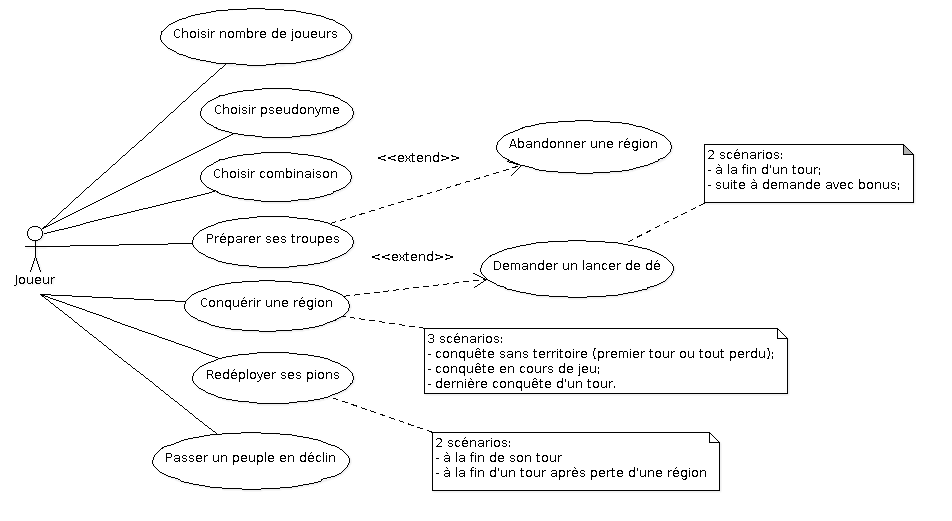
\includegraphics[width=16cm]{DiagrammeDeCasDUtilisation.png}\\
			\emph{Diagramme de cas d'utilisation}		
		\end{center}
		
		\newpage
		
		
		\subsection*{Annexe 2}
		
		\begin{center}
			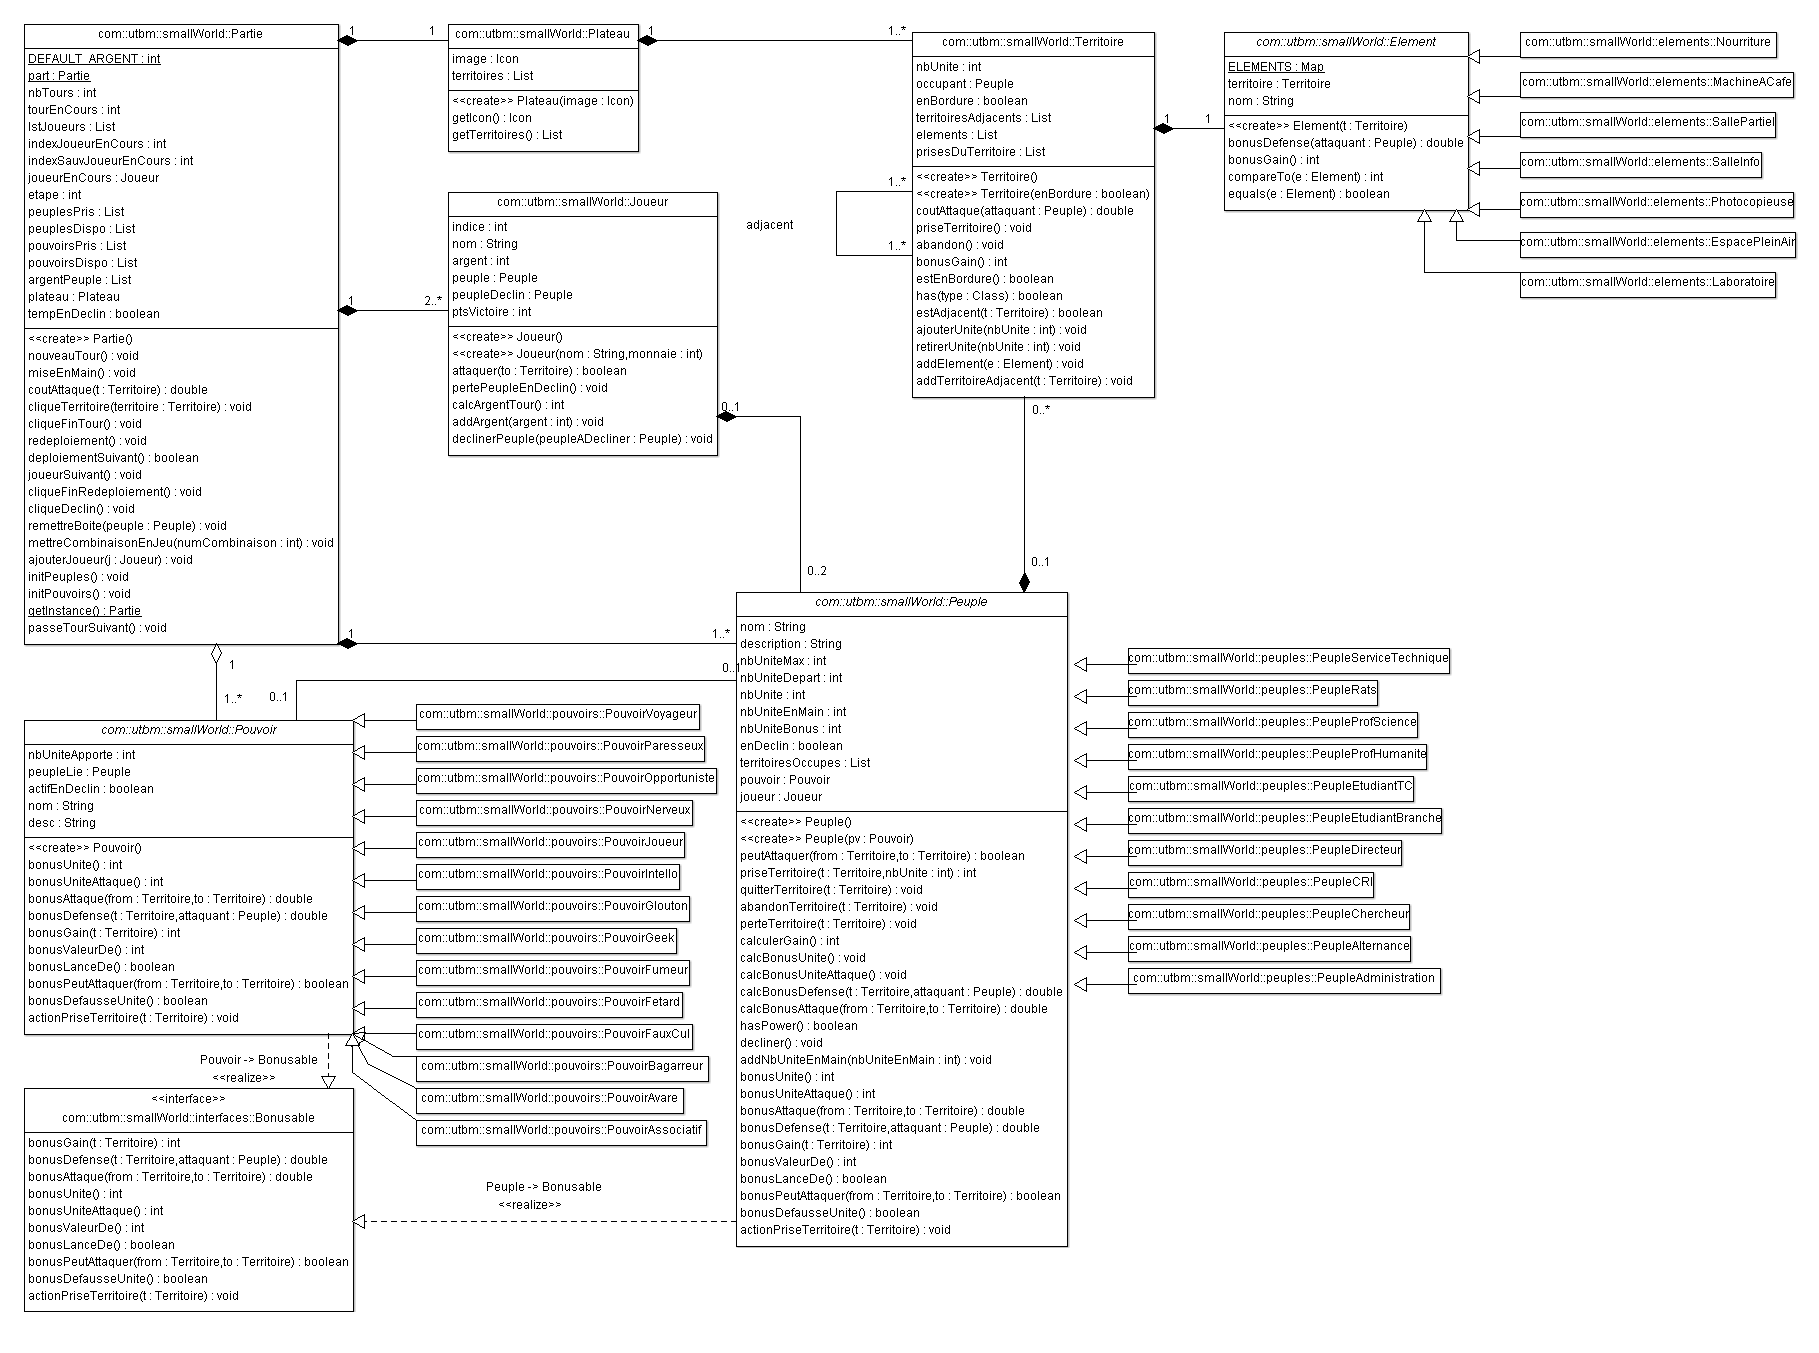
\includegraphics[width=16cm]{DiagrammeDeClasseAvecSub.png}\\
			\emph{Diagramme de classe général de l'application}		
		\end{center}
		
		\newpage
		
		\subsection*{Annexe 3}
		
		\begin{center}
			\includegraphics[width=15.7cm]{DSSAttaque2.png}\\
			\emph{Diagramme de séquences de l'attaque d'un territoire}
		\end{center}
		
		\newpage
		
		
		\subsection*{Annexe 4}
		
		\begin{center}
			\includegraphics[width=18cm]{DSSPriseTerritoireSansExistant.png}\\
			\emph{Diagramme de séquences de la prise d'un territoire sans occupant}
		\end{center}
		
		\newpage


		\subsection*{Annexe 5}
		
		\begin{center}
		\vspace*{3cm}
			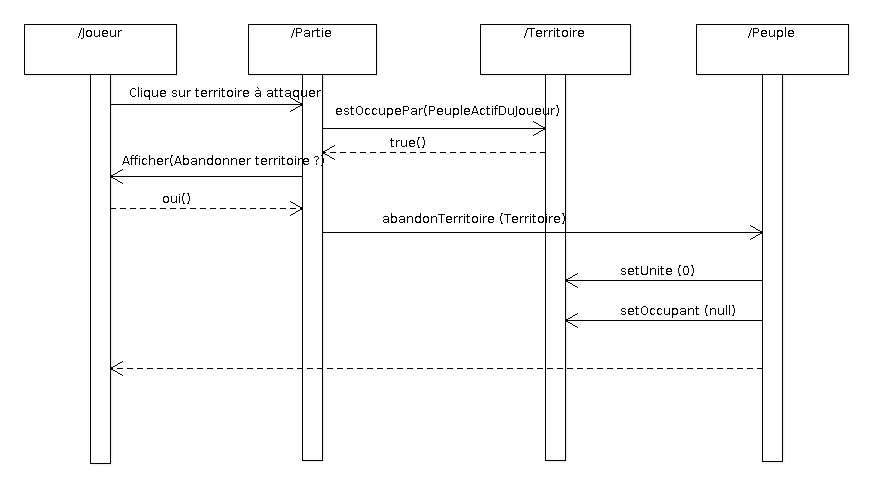
\includegraphics[width=9cm]{DSSAbandon.png}\\
			\emph{Diagramme de séquences de l'abandon d'un territoire}
		\end{center}
		
		\newpage


		\subsection*{Annexe 6}
		
		\begin{center}
			\includegraphics[width=9.5cm]{DSSCalculGain2.png}\\
			\emph{Diagramme de séquences du calcul du gain d'un joueur}
		\end{center}

		\newpage

		
	\end{appendix}
		
	\tableofcontents
		
\end{document}